\documentclass[10pt,letterpaper]{article}
% Author: Robert Warren

\usepackage[margin=19mm,headheight=14pt]{geometry}
\usepackage[T1]{fontenc}
\usepackage{lmodern}
\usepackage{xcolor}
\usepackage{graphicx}
\usepackage{hyperref}
\usepackage{fancyhdr}
\usepackage{longtable}
\usepackage{tabularx}
\usepackage{array}
\usepackage{listings}
\usepackage{enumitem}
\usepackage{microtype}

\definecolor{ink}{HTML}{17324D}
\definecolor{blue}{HTML}{1769AA}
\definecolor{pale}{HTML}{EFF5F9}
\definecolor{codebg}{HTML}{F3F5F7}
\definecolor{muted}{HTML}{526273}

\hypersetup{
  colorlinks=true,
  linkcolor=blue,
  urlcolor=blue,
  pdftitle={LaTeX Packages and Style Files: Complete Reference},
  pdfauthor={Robert Warren}
}
\pagestyle{fancy}
\fancyhf{}
\fancyhead[L]{\small\color{muted}LaTeX Packages and Style Files}
\fancyhead[R]{\small\color{muted}API reference}
\fancyfoot[C]{\small\thepage}
\renewcommand{\headrulewidth}{0.3pt}

\lstdefinestyle{tex}{
  language=[LaTeX]TeX,
  basicstyle=\ttfamily\small,
  keywordstyle=\color{blue}\bfseries,
  commentstyle=\color{muted},
  backgroundcolor=\color{codebg},
  frame=single,
  rulecolor=\color{pale},
  breaklines=true,
  keepspaces=true,
  columns=fullflexible,
  showstringspaces=false,
  xleftmargin=4pt,
  xrightmargin=4pt,
  aboveskip=6pt,
  belowskip=8pt
}
\lstset{style=tex}
\setlist{itemsep=2pt,topsep=3pt}
\setlength{\parindent}{0pt}
\setlength{\parskip}{5pt}
\renewcommand{\arraystretch}{1.16}
\newcolumntype{Y}{>{\raggedright\arraybackslash}X}
\newcommand{\pkg}[1]{\texttt{#1}}
\newcommand{\key}[1]{\texttt{#1}}
\newcommand{\optdefault}[1]{\textit{Default:} #1}

\title{\Huge\color{ink}LaTeX Packages and Style Files\\[4pt]
  \Large Complete Usage and Parameter Reference}
\author{Robert Warren}
\date{November 2026}

\begin{document}
\maketitle
\begin{center}
\large
This guide documents the included \pkg{RDFTools} and
\pkg{w3c-recommendation} packages, plus the optional external
\pkg{lua4ht} dependency used for direct HTML conversion.
\end{center}

\tableofcontents
\clearpage

\section{Scope and quick reference}

This distribution includes the two document-authoring packages shown below.
\pkg{lua4ht} is an optional external dependency for the documented direct
LuaLaTeX/TeX4ht HTML workflow; its package files are not included. The
optional internal \pkg{RDFTools-glossaries} bridge is loaded automatically
when glossary integration is requested; install it beside RDFTools.

\begin{longtable}{p{.23\linewidth}p{.29\linewidth}p{.39\linewidth}}
\textbf{Package} & \textbf{Primary purpose} & \textbf{Main entry points}\\
\hline
\pkg{RDFTools} & Display RDF source fragments and query registered RDF data. &
\verb|\useRDF|, \verb|rdfFragment|, \verb|\RDFTermName|, \verb|\citeBibo|\\
\pkg{w3c-recommendation} & W3C recommendation document layout and metadata. &
\verb|\WThreeCSetup|, \verb|\WThreeCTitlePage|, \verb|\WThreeCAbstract|\\
\pkg{lua4ht} & Optional external LuaLaTeX/TeX4ht HTML conversion dependency;
not bundled. & Install separately before using its HTML workflow.\\
\end{longtable}

Installable package files are under \verb|tex/latex/| and examples are under
\verb|doc/latex/|. The screenshots in this guide are rendered captures of
those examples, not mockups. This source, \texttt{style-reference.tex}, is
documentation to compile, not a \pkg{.sty} package to load.

\section{\pkg{RDFTools}}

\subsection{Purpose, dependencies, and loading}

\pkg{RDFTools} combines two APIs: source-fragment presentation and RDF-backed
reference lookup. Load it once in the preamble:

\begin{lstlisting}
\usepackage{RDFTools}
\end{lstlisting}

The package has no package-load options. Its reference API invokes the
bundled \pkg{RDFTools.lua} helper through trusted shell escape. The helper
requires TeX Live's \pkg{texlua}, LuaXML, and LuaSocket. HTTPS retrieval also
requires \pkg{curl}; HTTP-to-HTTPS redirects use it as well. Local sources and
plain HTTP do not require curl. Compile only trusted documents with shell
escape enabled.

For PDFLaTeX, enable shell escape explicitly when compiling by hand:
\begin{lstlisting}
pdflatex -shell-escape -interaction=nonstopmode -halt-on-error document.tex
\end{lstlisting}
The \verb|\useRDF| command checks for unrestricted shell escape and raises a
package error before attempting cache creation if this option is missing.
Without it, PDFLaTeX cannot run the parser helper or recreate a deleted
\texttt{rdfCache/} directory.

\subsection{RDF listing presentation}

\subsubsection{The \texttt{rdfFragment} environment}

\begin{lstlisting}
\begin{rdfFragment}[key=value,...]
  ...literal RDF text...
\end{rdfFragment}

\begin{rdfFragment}[source=examples/vocabulary.ttl,title={Vocabulary}]
  \caption[Short list entry]{Full fragment caption}
  \label{rdf:vocabulary}
\end{rdfFragment}
\end{lstlisting}

With no \key{source}, the environment prints the body as a verbatim,
line-numbered listing. With \key{source}, it imports and prints a local file.
An imported source must exist at the path supplied; this presentation
environment does not fetch URLs. A missing file raises a package error.
Rendered headings and caption labels use \emph{RDF Listing}, for example
\emph{RDF Listing 1: Vocabulary}. The environment name remains
\verb|rdfFragment|; existing documents and references do not need renaming.

\begin{longtable}{p{.19\linewidth}p{.18\linewidth}p{.54\linewidth}}
\textbf{Key} & \textbf{Default} & \textbf{Meaning}\\
\hline
\key{source} & empty & Local RDF/OWL file to display. Empty selects direct
verbatim content.\\
\key{title} & empty & Heading title and fallback entry in the list of RDF
fragments.\\
\key{label} & empty & LaTeX label attached to the fragment counter for
\verb|\ref|.\\
\key{caption} & empty & Caption text for a direct listing. In imported mode,
use the standard \verb|\caption| command inside the environment.\\
\key{format} & detected or direct-listing label & Explicit format label. It
overrides extension/content detection for imported sources and labels direct
listings. With no explicit format, a direct listing displays
\emph{Direct RDF listing} only if neither \key{title} nor \key{caption} is
provided. An explicit format remains visible with either option.
It does not convert or validate the source.\\
\key{show-source} & false & Show the imported file path below the heading.
Accepts a bare key for true, or \verb|show-source=false|.\\
\key{noprefix} & false & Hide Turtle/N3 \texttt{@prefix} and
SPARQL-style \texttt{PREFIX} declarations, including multiline declarations.
Accepts a bare key, \verb|noprefix=true|, or \verb|noprefix=false|.
Applies to imported files and direct listings; the original source is not
modified.\\
\end{longtable}

For example, to show the RDF content without prefix declarations:
\begin{lstlisting}
\begin{rdfFragment}[source=examples/vocabulary.ttl,noprefix]
  \caption{Vocabulary without prefix declarations}
\end{rdfFragment}
\end{lstlisting}
The option hides declaration lines rather than expanding prefixed names.
Base declarations, comments, and RDF content are retained. Omit the option
or use \verb|noprefix=false| to display the complete source.

For imported fragments, \verb|\caption{long text}| supplies the full caption;
\verb|\caption[short text]{long text}| uses the optional short text in the
list. The environment increments the \verb|rdfFragment| counter. The
printable names are customizable with \verb|\rdfname| and
\verb|\listofrdfname|; the counter representation is \verb|\therdfFragment|.
The default \verb|\rdfname| is \emph{RDF Listing}. The list heading remains
\emph{List of RDF fragments}; changing the rendered label does not rename
\verb|\listOfRDFfragments| or the counter. For example:
\begin{lstlisting}
\begin{rdfFragment}[title={Vocabulary extract},caption={Selected triples}]
ex:item ex:label "Example" .
\end{rdfFragment}
\end{lstlisting}
This prints the supplied title and caption without the redundant
\emph{Direct RDF listing} suffix. Adding \verb|format={Turtle}| explicitly
retains the \emph{Turtle} suffix.

\begin{figure}[htbp]
\centering
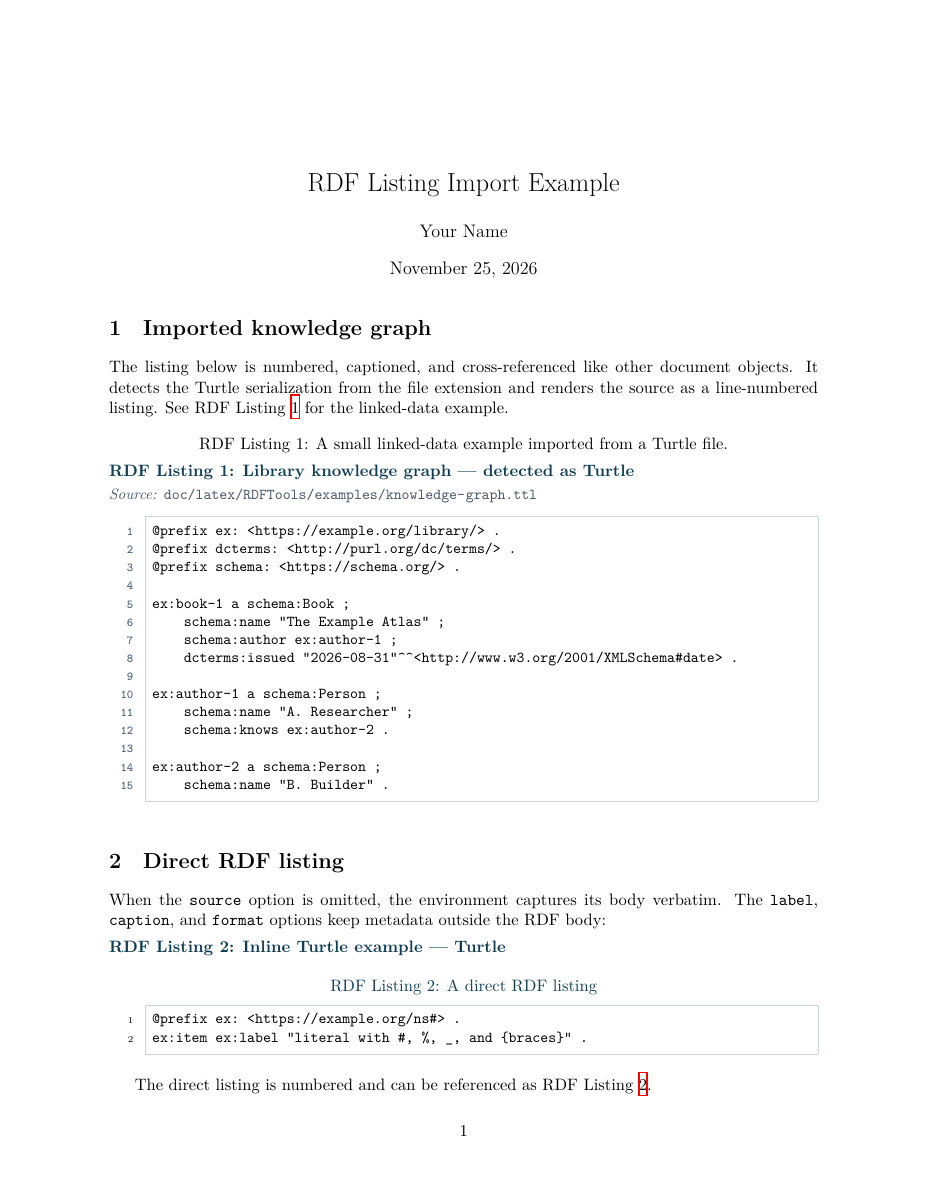
\includegraphics[height=.65\textheight,keepaspectratio]{screenshots/rdf-listing-example.png}
\caption{RDF listing headings, captions, and cross-references rendered by
the current package. The explicitly supplied Turtle format remains visible.}
\end{figure}

\subsubsection{Keeping an RDF listing on one page}

The \verb|rdfFragment| environment has no built-in keep-together or
automatic shrink-to-fit option. Use standard LaTeX page-layout tools around
the environment; both approaches below also work with imported listings.

\paragraph{Prefer keeping the listing together.}
Load \pkg{needspace} in the preamble, then reserve an estimated amount of
space immediately before the listing:
\begin{lstlisting}
% Preamble
\usepackage{needspace}

% Document
\Needspace{18\baselineskip}
\begin{rdfFragment}[title={Vocabulary extract},format={Turtle}]
@prefix ex: <https://example.org/> .
ex:Example a ex:Class .
\end{rdfFragment}
\end{lstlisting}
If less than the requested space remains, LaTeX starts a new page.
Adjust \verb|18\baselineskip| to include the listing body, heading,
caption, and surrounding spacing. This is an estimate, not a measurement
of the environment: the listing can still split if it needs more space.
It does not reduce the font size or scale the content. This is the
recommended approach when long listings must remain able to span pages.

\paragraph{Require a short listing to stay together.}
For a listing known to fit on one page, wrap the whole environment in a
\verb|minipage|:
\begin{lstlisting}
\par\noindent
\begin{minipage}{\linewidth}
\begin{rdfFragment}[title={Vocabulary extract},format={Turtle}]
@prefix ex: <https://example.org/> .
ex:Example a ex:Class .
\end{rdfFragment}
\end{minipage}
\par
\end{lstlisting}
LaTeX treats the block as unbreakable and moves it to the next page if
necessary. \textbf{Do not use this for a listing taller than a page:}
it cannot split and may extend beyond the bottom margin. No extra package
is required for \verb|minipage|. Neither approach makes the listing a float.

\subsubsection{Related fragment commands}

\begin{longtable}{p{.33\linewidth}p{.57\linewidth}}
\textbf{Command} & \textbf{Use}\\
\hline
\verb|\listOfRDFfragments| & Print the list of fragments. It uses a chapter
heading in book-like classes and a section heading otherwise.\\
\verb|\importRDFfragment{file}| & Shorthand for an imported
\verb|rdfFragment| with only the \key{source} key.\\
\verb|rdflisting[heading]| & Print arbitrary
verbatim text with the package's frame and line numbers. The optional heading
defaults to \emph{RDF fragment}.\\
\end{longtable}

The fragment format detector recognizes \texttt{.ttl}, \texttt{.n3},
\texttt{.nq}, \texttt{.nquads}, \texttt{.rdf}, \texttt{.xml}, and
\texttt{.owl}. For unknown extensions it inspects up to twenty lines for
serialization markers. Detection only affects the heading; the reference
extractor has its own supported syntax and validation rules.

\subsection{Registering a reference source}

\begin{lstlisting}
\useRDF[options]{document-prefix}{local-file-or-URL}
\useRDF{catalog}{examples/reference.ttl}
\useRDF[indexTerms]{catalog}{examples/reference.ttl}
\end{lstlisting}

The document prefix is an alias chosen by the author; it need not match a
prefix declared inside the RDF data. The second argument can be a local file
or an \texttt{http://} or \texttt{https://} URL. Calls queue sources for
preparation together near the end of the preamble. Parsed reference and
bibliography caches are regenerated for each compilation. For URLs, the
downloaded source response and response media type are reused when their
metadata matches the requested URL; RDFTools does not check the server for a
newer version on each run.
All RDFTools-generated caches and working files are stored in the automatically
created \texttt{rdfCache/} directory: parsed references, downloaded source
responses and their metadata, generated bibliography files, and term-index
working and sorted files. Original sources and normal LaTeX outputs
(including the \texttt{.rdfl} list-of-fragments auxiliary file) remain
in their usual locations. Update \texttt{RDFTools.sty},
\texttt{RDFTools.lua}, and \texttt{RDFTools-glossaries.sty} together;
older root-level caches are not migrated or used.

When compiling with Tectonic, run it with shell escape enabled and set
\texttt{-Z shell-escape-cwd} to the document's working directory, for example:
\begin{lstlisting}
tectonic -Z shell-escape -Z shell-escape-cwd="$PWD" document.tex
\end{lstlisting}
Without this setting, Tectonic runs helper commands in a temporary directory.
RDFTools may then be unable to find the Lua helper or a relative source file,
and the helper's \texttt{rdfCache/} will not be visible to LaTeX.

To refresh a downloaded ontology, remove its generated cache files from
\texttt{rdfCache/}:
\begin{itemize}
\item \texttt{<jobname>.rdfref.\allowbreak<prefix>.tex.source}: downloaded response;
\item \texttt{<jobname>.rdfref.\allowbreak<prefix>.tex.source.meta}: source URL metadata;
\item \texttt{<jobname>.rdfref.\allowbreak<prefix>.tex.source.type}: response media type.
\end{itemize}
Only remove generated cache files, not the original RDF sources. Changing
the URL also invalidates that source's downloaded response.

\subsubsection{Supported source formats and remote URLs}

The RDF reference API accepts local source files and HTTP/HTTPS URLs. It
recognizes these input formats by extension, response media type, or JSON
content:
\begin{longtable}{p{.30\linewidth}p{.58\linewidth}}
\textbf{Input} & \textbf{Parser}\\
\hline
\texttt{.ttl} or \texttt{text/turtle} & Turtle\\
\texttt{.n3} & N3 using the Turtle-compatible statement parser\\
\texttt{.nq}, \texttt{.nquads} & N-Quads\\
\texttt{.rdf}, \texttt{.xml}, \texttt{.owl}, or RDF/XML media type & RDF/XML\\
\shortstack[l]{\texttt{.jsonld}, \texttt{.json},\\JSON-LD media type or content} & JSON-LD\\
\end{longtable}

For remote URLs, RDFTools requests Turtle first, then RDF/XML, JSON-LD, and
JSON using HTTP content negotiation:
\begin{lstlisting}
Accept: text/turtle, application/rdf+xml;q=0.9,
        application/ld+json;q=0.8, application/json;q=0.7
\end{lstlisting}
The final response media type selects the parser, including after redirects.
If no useful media type is supplied, a recognized filename extension selects
the format; the JSON-LD media types are \texttt{application/ld+json} and
\texttt{application/json}. Downloaded content, its source URL, and response
media type are cached under \texttt{rdfCache/}.
HTML responses are rejected rather than parsed as RDF. In particular,
\url{https://schema.org/} is an HTML page, not the vocabulary export; use the
Turtle or JSON-LD download URL shown in the following sections.

\subsubsection{Turtle literals and whole-vocabulary exports}

Turtle sources support single- and double-quoted strings, including
multiline triple-quoted forms, with language tags and datatype suffixes.
For example:
\begin{lstlisting}
ex:Example rdfs:comment """A multiline definition.
# This line belongs to the definition, not a comment.
The words GRAPH and @forAll are ordinary text here."""@en .
\end{lstlisting}
Quotes, comment markers, periods, and directive-looking lines inside a
long literal are retained as text. Graph keywords embedded in identifiers
such as \texttt{PROTECTED\_GEOGRAPHICAL\_INDICATION} no longer cause a
false syntax error. Actual graph blocks, N3 quantification, and Turtle
collection shorthand remain unsupported.

Use explicit machine-readable whole-vocabulary exports rather than
human-readable term pages:
\begin{lstlisting}
\useRDF[glossary=used]{schema}{
  https://schema.org/version/latest/schemaorg-current-https.ttl
}
\useRDF[glossary=used]{gs1}{
  https://ref.gs1.org/voc/data/gs1Voc.ttl
}
\end{lstlisting}
Loading these exports does not automatically follow imports, combine
separate sources for hierarchy traversal, or equate HTTP and HTTPS
resource identifiers. The Schema.org JSON-LD export is also supported:
\begin{lstlisting}
\useRDF{schema}{
  https://schema.org/version/latest/schemaorg-current-https.jsonld
}
\end{lstlisting}

\subsubsection{JSON-LD sources}

JSON-LD supports inline JSON-LD 1.1 contexts and context arrays; term and
prefix mappings; \texttt{@base}, \texttt{@vocab}, and \texttt{@language};
term-level \texttt{@type} and \texttt{@language}; \texttt{@id},
\texttt{@type}, \texttt{@graph}, \texttt{@included}, nested node objects,
value objects, language-tagged and typed literals, strings, numbers,
booleans, and \texttt{@list} collections.
For example, an inline context maps the short \texttt{schema:} prefix and
gives the literal name a language tag:
\begin{lstlisting}
{
  "@context": {
    "schema": "https://schema.org/",
    "name": {"@id": "schema:name", "@language": "en"}
  },
  "@id": "schema:Product",
  "name": "Product"
}
\end{lstlisting}

For safety, remote \texttt{@context} URLs and \texttt{@import} are rejected;
RDFTools does not fetch context documents. Scoped or nested term definitions
(\texttt{@context}, \texttt{@nest}) and reverse properties
(\texttt{@reverse}) are unsupported. JSON input is limited to 8 MiB, nested
values to 128 levels, and inline context application to 32 levels. The
implementation covers these documented forms, not the full JSON-LD 1.1
specification. Context prefixes are retained for lookups. If namespaces share
a local name, RDFTools prefers the unique namespace matching the
\verb|\useRDF| source prefix; otherwise use the context-prefixed name or full
URI to avoid ambiguity.

\subsubsection{Memory and repeated lookups}

The helper prepares all registered sources in one batch, reducing helper
startup overhead. It still writes one parsed cache per source. Lookup commands
stream those cache files rather than loading all ontology records into
persistent TeX lists. A bounded cache retains at most 32 recent lookup results,
including hierarchy lists; when full, new results replace older entries.
Repeated references that hit this cache avoid rescanning their source, while
references whose results have been replaced scan the corresponding cache
again. This trades some compile time for lower retained TeX memory as ontology
counts increase.

Glossary preparation has a separate memory cost. For compatibility with
\verb|\makenoidxglossaries|, entries must be defined in the preamble.
\key{glossary=used} records referenced IDs on disk and, on the next run,
streams the source cache to define only those entries. Its TeX entry memory
therefore follows the number of referenced terms rather than every term in
the ontology. \key{glossary=full} still defines every named term.

Run the included PDFLaTeX benchmark from this directory:
\begin{lstlisting}
python3 ../RDFTools/benchmark_rdf_memory.py --terms 1000 --ontologies 1 2 4
\end{lstlisting}
A recent run measured peak RSS of 56.0, 55.8, and 56.1 MB for one, two, and
four synthetic ontologies. These are example process measurements, not
guarantees; engine, TeX distribution, source shape, and glossary mode affect
the result. The benchmark also reports compile time. Add \texttt{--no-lookups}
to isolate preparation, or select \texttt{--glossary full} or
\texttt{--glossary used} to measure glossary cost; used mode measures two
PDFLaTeX passes. A synthetic 10{,}000-term source with one referenced term
compiled at 66.6 MB peak RSS in used mode on this machine.

For RDF/XML, internal literal entities (including the URI entities used by
OMG Commons) are supported with bounded expansion. External DTDs, external
entities, parameter entities, and entity replacement markup are rejected;
no external entity resources are fetched. Expansion is limited to 16 nested
references, 1 MiB of replacement text per expansion, and 8 MiB of expanded
ordinary XML content. Comments and CDATA retain literal entity references.

The parser resolves inherited \texttt{xml:base}, relative IRIs, and
\texttt{rdf:ID}, and handles nested resource nodes.
For \texttt{rdf:parseType}, both \texttt{Resource} and \texttt{Collection}
are supported. Collections preserve member order, including anonymous
resources; an empty collection becomes \texttt{rdf:nil}. This supports
FIBO union and property-chain lists. The \texttt{Literal} parse type
remains unsupported and produces an error.
Superclass and superproperty lists omit anonymous restriction nodes and list
only named parents.

\begin{longtable}{p{.25\linewidth}p{.62\linewidth}}
\textbf{Option} & \textbf{Meaning}\\
\hline
\key{indexTerms} & Bare option or \verb|indexTerms=true| enables collection of
referenced terms for the term index. \verb|indexTerms=false| disables it.
Default: false.\\
\key{glossary} & \texttt{full} includes all defined terms;
\texttt{used} includes referenced terms; \texttt{none} disables integration.
Default: \texttt{none}. A bare option selects \texttt{full}.\\
\end{longtable}

\subsection{Integration with the glossaries package}

\begin{lstlisting}
\usepackage[french]{babel} % choose the document language
\usepackage{RDFTools}
\usepackage[nonumberlist]{glossaries}
\makenoidxglossaries
\useRDF[glossary=used]{vocab}{vocabulary.ttl}

\begin{document}
\RDFTermName{vocab}{Report}
\RDFTermDefinition{vocab}{Report}
\printnoidxglossary[title={RDF Terms}]
\end{document}
\end{lstlisting}

With PDFLaTeX and the no-index workflow, compile at least three times: one
run discovers references, the next prepares their glossary definitions, and
the third prints the glossary from the updated auxiliary data. A newly used
term has unlinked text until its entry is prepared, and RDFTools requests a
rerun in the log. Tectonic may perform these passes automatically. With
\verb|\makeglossaries|, compile twice before running \texttt{makeglossaries},
then compile again.

The \key{glossary=full} mode includes all named subjects defined in the source,
excluding anonymous nodes and the \texttt{owl:Ontology} metadata resource.
The \key{glossary=used} mode selects terms referenced by
\verb|\RDFTermName|, \verb|\RDFTermDefinition|, \verb|\RDFTermURI|,
\verb|\RDFListSuper|, or \verb|\RDFListSuperTransitive|.
Hierarchy commands select the queried resource as well as the parents they
display. Aliases, repeated calls, and multiple source prefixes for the same
resource share one entry in the main glossary.

When glossary integration is enabled for a source, \verb|\RDFTermName| and
\verb|\RDFTermDefinition| make their existing output a hyperlink to that
term's glossary entry. Each parent printed by \verb|\RDFListSuper| or
\verb|\RDFListSuperTransitive| links individually to its own entry;
localized labels and comma/\emph{and} formatting are unchanged.
\verb|\RDFTermURI| instead behaves as an external \verb|\href| to the full
resource URI, with the existing \texttt{prefix:term} display text. It still
selects the resource in \key{glossary=used} mode. Aliases use the same glossary
destination. Disabled sources and resources without entries keep their
unlinked lookup text. Print the glossary as usual to create link destinations.

Entries show the definition, a clickable full URI, and all named ancestors
under separate \textbf{Superclasses} and \textbf{Superproperties} headings.
The full URI itself is typeset with \verb|\small|; the \textbf{URI:} label,
definition, and ancestor lists retain their normal text size.
Ancestors use the RDF source's \texttt{prefix:term} notation, linked to their
full resource URIs. The most specific matching namespace is used; an
unmatched URI is displayed in full. A default namespace uses \texttt{:term}.
Equally specific namespace aliases use the first declared prefix. These are
the RDF source's namespace prefixes, not the author-chosen registration
alias: registering a source as \texttt{vocab} can therefore yield ancestors
such as \texttt{ex:Document} and \texttt{ex:Resource}.
Empty hierarchy sections are omitted. Ancestor metadata does not select additional glossary entries
in \key{glossary=used} mode.

RDF entries suppress the glossary style's automatic trailing punctuation,
so the definition's own punctuation is not doubled. Manually defined
glossary entries retain their existing style and punctuation.

Glossary names and definitions use the document language at the end of the
preamble, with the existing language and predicate fallbacks. A per-command
language override affects that command's output only. A missing label falls
back to the resource's local name. A missing definition displays
\texttt{No definition available.} and produces a warning once when selected.
Missing name, definition, and URI lookups retain their usual warnings and do
not create glossary entries. Both hierarchy commands warn when the requested
term is unknown. A valid term with no named parents returns no output without
a warning.

Definitions are prepared in the preamble for compatibility with
\verb|\makenoidxglossaries|. \key{glossary=full} prepares all named resources;
\key{glossary=used} prepares only IDs recorded in the previous run's
\texttt{rdfCache/\allowbreak<jobname>.rdfused.tex} file. Register sources and
configure languages before \verb|\begin{document}|. For a resource present
in several sources, the first registered definition takes precedence.
Glossary integration is independent of \key{indexTerms}; omitting the option
on another source leaves that source disabled.

The bridge loads \pkg{glossaries} automatically when needed. Load
\pkg{glossaries} explicitly first to supply its package options, and configure
it with \verb|\makenoidxglossaries| or \verb|\makeglossaries| as usual.
The indexed workflow uses \verb|\printglossary| and requires the normal
external glossary-indexing step; RDFTools does not run that indexer.
Use \verb|\printglossary[title={RDF Terms}]| for the same heading in that
workflow. The heading is supplied by the document's print command, rather
than imposed globally on manually defined glossaries.
Glossaries' auxiliary files follow its own output settings, while RDFTools
caches remain in \texttt{rdfCache/}.

Build the complete example with
\texttt{make -C latex glossary-example}. Its source is
\texttt{../RDFTools/\allowbreak rdf-glossary-example.tex}.

\begin{figure}[p]
\centering
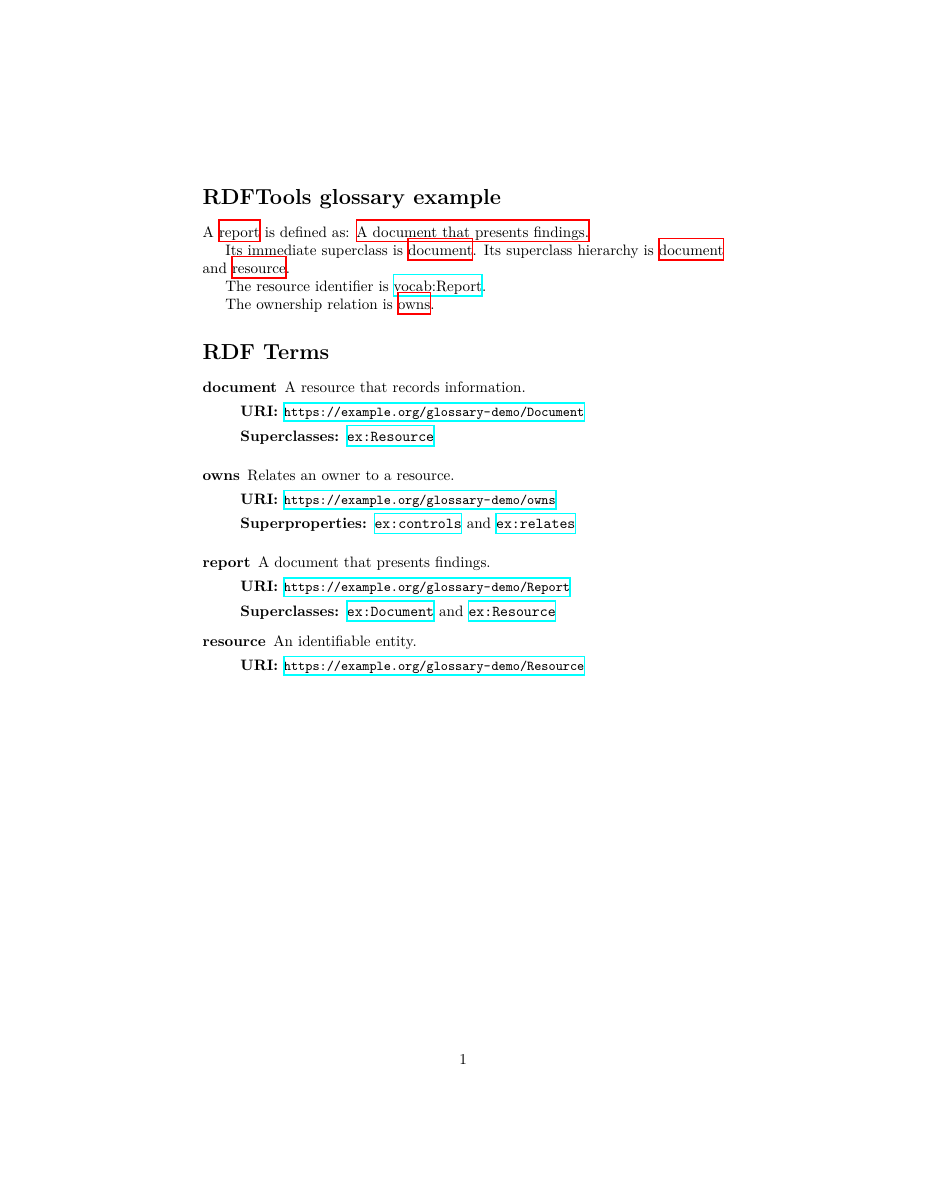
\includegraphics[height=.72\textheight,keepaspectratio]{screenshots/rdf-glossary-example.png}
\caption{Current RDF glossary rendering: the RDF Terms heading, definitions
without duplicate trailing punctuation, full term URIs, and linked
\texttt{prefix:term} identifiers for all superclass and superproperty ancestors.}
\end{figure}

\subsection{Term, URI, and ontology metadata commands}

Each resource may be addressed by its local name, a declared prefixed alias,
or its full IRI (without angle brackets).

The five term commands accept both \texttt{\{vocabulary\}\{term\}} and the
single-argument \texttt{\{vocabulary:term\}} form. Existing two-argument calls
remain supported, and the forms can be mixed freely:
\begin{lstlisting}
\RDFTermName{vocab:Report}
\RDFTermName{vocab}{Report} % equivalent
\RDFTermDefinition{vocab:Report}[fr][CA]
\RDFListSuper{vocab:Report}
\RDFListSuperTransitive{vocab:Report}
\RDFTermURI{vocab:Report}
\end{lstlisting}
The vocabulary is the alias registered by \verb|\useRDF|. Only the first
colon separates vocabulary and term. Thus \verb|{vocab:ex:Report}| selects
the \texttt{ex:Report} alias, and
\verb|{vocab:https://example.org/Report}| selects a full IRI within
\texttt{vocab}. Neither component may be empty. Both forms preserve glossary
selection and links, external URI hyperlinks, warnings, and term indexing.
The table below shows the original form; the compact alternative applies to
its first five commands, not to the ontology metadata commands.

\begin{longtable}{p{.3\linewidth}p{.25\linewidth}p{.33\linewidth}}
\textbf{Command} & \textbf{Parameters} & \textbf{Result}\\
\hline
\verb|\RDFTermName{prefix}{term}| &
prefix, term; optional \verb|[language]| or \verb|[language][region]| &
Preferred label literal. Predicates: \texttt{skos:prefLabel},
\texttt{foaf:name}, then \texttt{rdfs:label}.\\
\verb|\RDFTermDefinition| &
prefix, term; optional language/region brackets &
Definition literal. Predicates: \texttt{skos:definition}, then
\texttt{rdfs:comment}.\\
\verb|\RDFListSuper{prefix}{term}| & prefix, class or property term &
Immediate \texttt{rdfs:subClassOf} or \texttt{rdfs:subPropertyOf} parents,
rendered as localized term names.\\
\texttt{\textbackslash RDFListSuper\allowbreak Transitive\{prefix\}\{term\}} &
prefix, class or property term &
All transitive superclasses and/or superproperties, rendered as localized
term names.\\
\verb|\RDFTermURI{prefix}{term}| & prefix, term &
Hyperlink to the full IRI, displayed as \texttt{prefix:term}.\\
\verb|\RDFTitle{prefix}| & registered source prefix; optional
\verb|[language]| or \verb|[language][region]| &
Title for the ontology or vocabulary.\\
\verb|\RDFName{prefix}| & registered source prefix; optional language/region &
Source/ontology name.\\
\verb|\RDFVersion{prefix}| & registered source prefix &
Version metadata.\\
\end{longtable}

The optional single bracket may hold a combined tag, for example
\verb|[fr-CA]|. The two-bracket form \verb|[fr][CA]| is equivalent. A
lowercase two-letter value is treated as a language; an uppercase two-letter
value is treated as a region. An exact language-region match is preferred,
then a matching language or region, English, and finally an untagged value.
Predicate priority is also applied for names and definitions.
Language brackets follow the required arguments, for example:
\begin{lstlisting}
\RDFTermName{vocab}{Report}[fr]
\RDFTermName{vocab:Report}[fr]
\RDFTermDefinition{vocab}{Report}[fr][CA]
\RDFTermDefinition{vocab:Report}[fr][CA]
\RDFTitle{vocab}[fr-CA]
\RDFName{vocab}[fr]
\end{lstlisting}
The hierarchy commands have no language arguments; their individual
\verb|\RDFTermName| calls use the normal default lookup selection.

Lookup commands preserve source whitespace after the complete command,
including after optional language/region brackets. Thus a following word
does not run into the label or definition. The same rule applies to
\verb|\RDFTitle| and \verb|\RDFName|. A single source line break acts like a
normal space; whitespace before an optional bracket is syntax and is not
printed. No space is invented before punctuation or an intentional suffix:
\begin{lstlisting}
\RDFTermName{vocab:Report} describes the findings.
\RDFTermName{vocab}{Report}[en] describes the findings.
\RDFTermName{vocab:Report}, followed by a comma.
\RDFTermName{vocab:Report}.
\end{lstlisting}
Both reference forms and glossary-enabled output follow the same spacing
rules. Ordinary words require no empty-group or explicit-space workaround.

If no value is found, the lookup emits a \verb|Package RDFTools Warning| in
the LaTeX log and returns \texttt{Undefined}. URI lookup warns and returns an
empty URI, which is displayed as \texttt{Undefined}. Missing references are
still recorded when \key{indexTerms} is enabled.

\verb|\RDFListSuper{prefix}{term}| lists only immediate parents.
\verb|\RDFListSuperTransitive{prefix}{term}| follows both
\texttt{rdfs:subClassOf} and \texttt{rdfs:subPropertyOf} links transitively;
direct parents appear first, followed by more distant ancestors in source
order. Each name is produced by \verb|\RDFTermName| using the default language
selection. Items are separated by commas, with \emph{and} before the final
item. A term with no parents produces no output.

\subsection{BIBO bibliography API}

\begin{lstlisting}
\useRDF{bibo}{examples/bibliography.ttl}
The article is cited here: \citeBibo{bibo}{paper}.
\end{lstlisting}

\verb|\citeBibo{prefix}{resource}| cites a resource typed with a recognized
BIBO class. The second argument can be any stored alias for the resource.
Citation keys are deterministic and aliases/repeated calls point to one entry.
The helper creates
\texttt{rdfCache/\allowbreak<jobname>.rdfref.\allowbreak<prefix>.bib};
it never edits a
user-owned bibliography file.

With \pkg{biblatex}, generated bibliography files are registered as resources.
With \pkg{natbib} or classic BibTeX, the generated bibliography file is
appended to the normal bibliography list. If neither \pkg{biblatex} nor
\pkg{natbib} is loaded, the classic BibTeX interface is used with a warning.
An unknown BIBO resource also produces a package warning and displays
\texttt{Undefined}.

The extractor maps common BIBO classes to BibTeX entry types and extracts
authors/editors, title, publisher, journal, volume/number/pages, date/year,
DOI, ISBN/ISSN, URL, abstract, note, edition, series, chapter, and
organization. It expands explicit \texttt{rdf:first}/\texttt{rdf:rest} lists
and RDF/XML collections, including ordered BIBO author lists.
Turtle collection shorthand remains unsupported and is rejected rather than
guessed.

\texttt{\textbackslash RDFReferenceBib\allowbreak File\allowbreak\{prefix\}} expands to
the generated bibliography filename for one prefix.
\texttt{\textbackslash RDFReferenceBib\allowbreak Files} expands to the current
comma-separated list of registered generated bibliography files.

\subsection{RDF term index}

\verb|\makeRDFIndex| prints the term index at the point where it appears in
the document. Enable collection with \verb|\useRDF[indexTerms]{...}{...}|.
The current run writes
\texttt{rdfCache/\allowbreak<jobname>.rdfidx.new}; the helper sorts and
deduplicates it into \texttt{rdfCache/\allowbreak<jobname>.rdfidx}
at end of document. As with a
table of contents, compile again to display newly collected entries. Entries
are ordered case-insensitively by term, then by prefix, and PDF/HTML anchors
link back to the first use.

\begin{figure}[p]
\centering
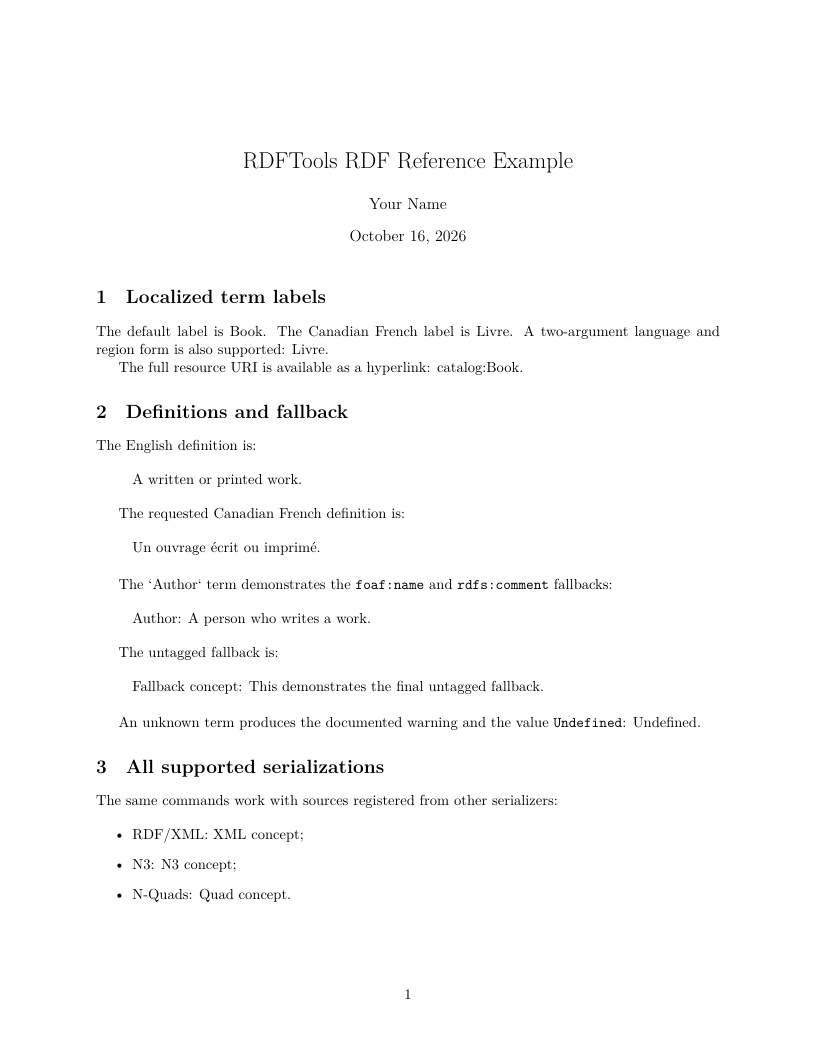
\includegraphics[height=.72\textheight,keepaspectratio]{screenshots/rdf-tools-example.png}
\caption{Rendered RDFTools reference example: localized names and
definitions, URI link, missing-term fallback, and multiple serializations.}
\end{figure}

\section{\pkg{w3c-recommendation}}

\subsection{Purpose and document setup}

Load the package in an article-like document. It sets page geometry,
hyperlink colors, headers/footers, heading typography, and a W3C-style title
page. It replaces \verb|\maketitle| with \verb|\WThreeCTitlePage|.

\begin{lstlisting}
\usepackage{w3c-recommendation}
\WThreeCSetup{
  title={RDF 1.2 Concepts},
  status={Working Draft},
  date={16 October 2026},
  editors={Example Editor}
}
\begin{document}
\WThreeCStart
\maketitle
\WThreeCContents
\WThreeCAbstract{Abstract text.}
\WThreeCStatus{Publication status text.}
% ordinary \section, \subsection, and document content
\WThreeCEnd
\end{document}
\end{lstlisting}

There are no package-load options. Configure metadata with
\verb|\WThreeCSetup{key=value,...}|. All setup keys are optional.

\begin{longtable}{p{.26\linewidth}p{.66\linewidth}}
\textbf{Setup key} & \textbf{Use and output}\\
\hline
\key{title} & Main title; also sets LaTeX's \verb|\title|. Default:
\emph{Untitled Recommendation}.\\
\key{subtitle} & Subtitle below the title.\\
\key{status} & Publication status and HTML status ribbon. Default:
\emph{Working Draft}.\\
\key{date} & Display date. Default: \verb|\today|.\\
\key{version} & Version URL shown below the title.\\
\key{latest} & Latest published version URL, preceded by
\key{latest-label}.\\
\key{editors} & Editor names/affiliations.\\
\key{feedback} & Feedback link or text.\\
\key{organization} & Organization metadata.\\
\key{documentnumber} & Document identifier.\\
\key{copyright} & Copyright line and HTML footer content.\\
\key{logo} & Path to a logo image. If the file is absent, the value is shown
as text; with no value, the package displays a W3C text mark.\\
\key{shortname} & Stored short-name metadata for the document.\\
\key{language-code} & HTML \texttt{lang} value on the outer document shell.\\
\key{toc-label} & Table-of-contents/sidebar label. Default:
\emph{Table of Contents}.\\
\key{abstract-label} & Abstract heading. Default: \emph{Abstract}.\\
\key{status-label} & Status-section heading. Default:
\emph{Status of This Document}.\\
\key{latest-label} & Label before the \key{latest} URL.\\
\key{details-label} & Summary label for \verb|\WThreeCMoreDetails|.\\
\key{editors-label} & Label for editor metadata.\\
\key{feedback-label} & Label for feedback metadata.\\
\key{organization-label} & Label for organization metadata.\\
\key{documentnumber-label} & Label for document number metadata.\\
\key{language-links-label} & Accessible label for the language links nav.\\
\end{longtable}

\subsection{Commands and parameters}

\begin{longtable}{p{.39\linewidth}p{.5\linewidth}}
\textbf{Command} & \textbf{Parameters and behavior}\\
\hline
\verb|\WThreeCSetup{keys}| & Apply document-wide metadata keys from the table
above.\\
\verb|\WThreeCLanguageSetup{language}{keys}| & Store a translated set of
metadata values under a language name, usually the Babel language name such
as \texttt{english} or \texttt{french}. Uses the same setup keys.\\
\verb|\WThreeCSelectLanguage| & Select profile from Babel's active
\verb|\languagename|.\\
\verb|\WThreeCSelectLanguage[language]| & Select a named language profile
explicitly.\\
\verb|\WThreeCLanguageLink{label}{url}| & Add a language-version link. It is
emitted in HTML mastheads and omitted from PDF output.\\
\verb|\WThreeCStart| & Open the HTML status ribbon/sidebar/main-content
wrappers. No output in PDF mode. Call near the start of the document.\\
\verb|\maketitle|, \verb|\WThreeCTitlePage| & Render title, status, version,
logo, editors, feedback, organization, document number, and copyright.\\
\verb|\WThreeCContents| & Print the PDF table of contents. In HTML, the
contents are placed in the sidebar by \verb|\WThreeCStart|.\\
\verb|\WThreeCAbstract{text}| & Render the abstract section; text is the
single required argument.\\
\verb|\WThreeCStatus{text}| & Render the status section; text is the single
required argument.\\
\verb|\WThreeCMoreDetails{text}| & Render collapsible HTML details or a
labelled quotation in PDF.\\
\verb|\WThreeCEnd| & Close the HTML main-content wrapper and emit the footer.
No output in PDF mode. Call at the end of the document.\\
\end{longtable}

The package uses ordinary \verb|\section|, \verb|\subsection|, and
\verb|\subsubsection| commands with its own colors and spacing. Profile
selection occurs at document start; configure profiles in the preamble and
activate the appropriate Babel language before the document begins. The HTML
navigation/layout is enabled when TeX4ht's \verb|\HCode| is defined.

\begin{figure}[p]
\centering
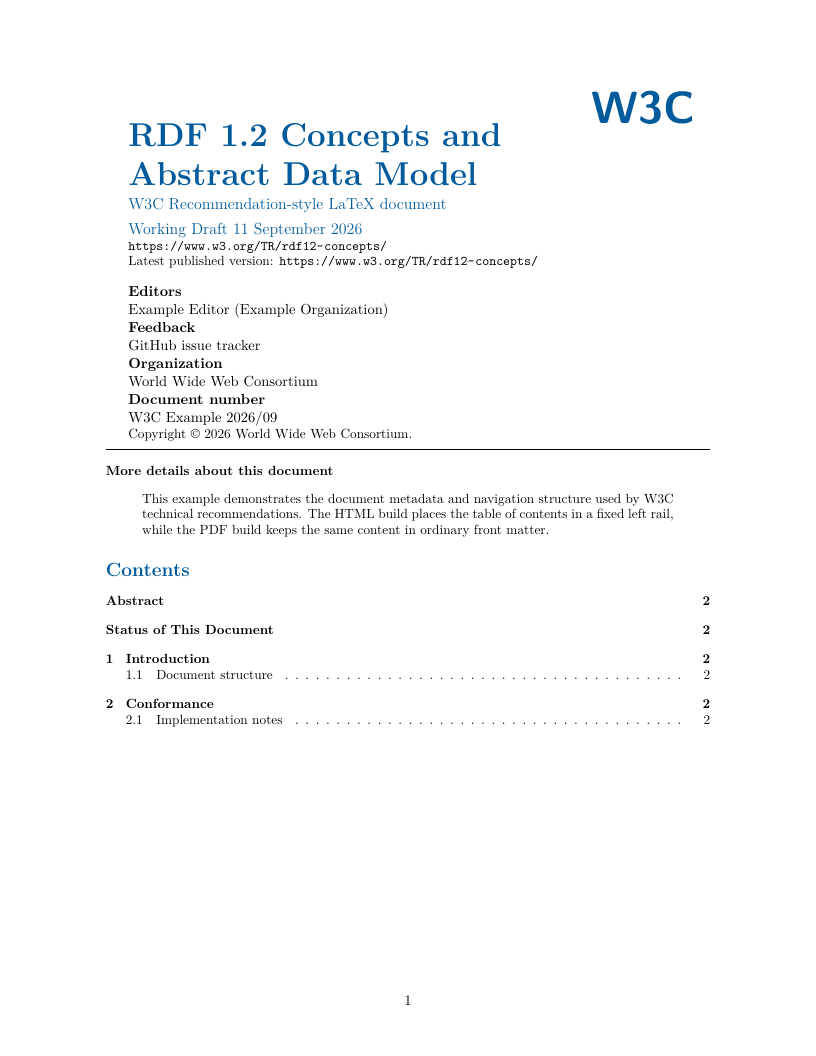
\includegraphics[height=.72\textheight,keepaspectratio]{screenshots/w3c-recommendation-example.png}
\caption{PDF rendering of the W3C recommendation style, including the
masthead, metadata, and table of contents.}
\end{figure}


\end{document}
